\chapter{Lecture 6}
\lhead{January 26, 2015}
\chead{21-366 Lambda Calculus Lecture 6}

\def\uwavy#1{#1}

\section{Computing With $\l$ Terms}
To perform computations, we need data structures. How do we represent data structures? We can use collections of terms that look like data structures. Our target for this lecture is to define the nonnegative integers, booleans, and finite sets. Once we have described these data structures, we can define some operations on them. Specifically, we will define addition and subtraction for the integers, and the conditional operator which branches between two terms dependant on whether a boolean is true or false.

\section{Data Structures}

\subsection{Booleans}
\index{Boolean|textbf}
The way that we define booleans at first may seem a little bit strange. The reason that we define them in the way that we do is motivated by the common use cases for booleans. Often, we want to use booleans inside conditional statements, to decide which of two branches to take. We might write, for example, the following program:
\begin{center}
  \begin{lstlisting}[language=C,backgroundcolor=\color{txtbkpaleblue},showstringspaces=false]
    int age = keyboard.read();
    if (age >= 21) {
      print("Welcome to the bar!");
    }
    else {
      print("Come back when you are older.");
    }
  \end{lstlisting}
\end{center}

One way to do this is to establish an application $(XY)$ where $X$ is the term you would like to evaluate in the case where your boolean is true, and $Y$ is the term you would like to evaluate in the case where your boolean is false.\\

So, in our above example, we would have a term representing the function \texttt{print("Welcome to the bar!")} as $X$ and \texttt{print("Come back when you are older.")} as $Y$. We could then represent the booelan true as the function $(\l xy.x)$ and the boolean false as the function $(\l xy.y)$. We define $K := \l xy.x$ as our true boolean, and $K_* := \l y.xy$ as our false boolean.\\

Typically, if we have some term $T$, we write $T_* := TI$. This is where our notation for $K_*$ is derived. We can demonstrate that $K_* =_\beta KI$ by $\beta$ conversion:
\begin{equation*}
  KI = (\l xy.x)I \rightarrow_\beta Iy = (\l yI) =_\beta \l y\l zz =_\beta \l yz.z =_\alpha \l xy.y = K_*
\end{equation*}

\subsection{Integers}
\index{Integer|textbf}
The integers are substantially more difficult to represent than booleans. We need some manner of term which can be straightforwardly added, subtracted, and so on. When you factor in the possibility of negative numbers, the difficulty becomes unnecessarily high for an introductory work. So we will restrict ourselves to the nonnegative integers $0,1,2,\ldots$. To avoid confusion, we will write conventional numbers as usual, and numbers which we mean to be represented by our integer data structure with an underline, as in $\uline{n}$.\\

A good starting point is to consider the most simple problem which we face with our integer representation: counting. If our technique for incrementing an integer by one is complicated, it is a sign that the rest of our representation will be even more so. One way that we can represent numbers which turns out to be very nice for incrementing is to take some arbitrary term $a$ and repeat it $n$ times. These numbers are called the \textbf{Church numerals}\index{Church,Alonzo!Church Numerals}.\\

\begin{equation*}
  \uline{n} = \underbrace{a \cdot a \cdot ... \cdot a}_{n\hbox{ times}} = a^n
\end{equation*}

This is a nice, clean representation of the number $n$. One downside is that it fails fairly catastrophically for all numbers less than $1$. Usually, we would write that $a^0 = 1$, but $1$ does not have meaning in the context of repeating a term $a$. $a^{-n} = 1 / a^n$ is even worse, from the standpoint of lambda expression representation. This is why we ignore negative numbers for now.\\

The solution to the problem of representing zero is actually fairly simple. We can just declare that $a^1 = 0, a^2 = 1$, and so on. So we in fact have that:\\

\begin{equation*}
  \uline{n} = \underbrace{a \cdot a \cdot ... \cdot a}_{n+1\hbox{ times}} = a^{n+1}
\end{equation*}

All that we are missing now is the actual term which represents zero. For this, we will use $K_*$. Ordinarily, we would try to motivate this choice and explain in some way why we made the decision. For now, we will have to satisfy ourselves with the knowledge that the decision will make some complicated constructions more simple down the line.\\

We now know enough to write a general version of the number $\uline{n}$ as a term. Notice that our term is not precisely a term applied to itself over and over again. Our analogy to exponentiation of a number $a$ motivates our strategy, but is not perfect.\\

\begin{equation*}
  \uline{n} := \l xy . (\underbrace{x(x(\ldots x}_{n}y))\ldots)
\end{equation*}

\margnot{A Few Church Numerals}{ 
  \begin{eqnarray*}
    \uline{0} &=& \l xy.y\\ 
    \uline{1} &=& \l xy.xy\\ 
    \uline{2} &=& \l xy.xxy\\ 
    \uline{3} &=& \l xy.xxxy\\ 
    \uline{4} &=& \l xy.xxxxy\\
    &\ldots&
    \end{eqnarray*}
}

The next step down our rode to addtion is a function $\uline{s}$ which takes a number $\uline{n}$ to a number $\uline{n+1}$. We call this function \textbf{successor}\index{Successor Function}. In our function notation, we write that:

\begin{equation*}
  \uline{S}\ \uline{n} \twoheadrightarrow_\beta \uline{n + 1}.
\end{equation*}

The definition of the function $S$ follows naturally from the definition of the Church numerals. We simply want to add another $x$ to the chain.
\begin{equation*}
  \uline{S} := \l nxy.x((n x) y) 
\end{equation*}

\examplebox{Example: Applying $\uline{S}$ to $\uline{0}$ to get $\uline{1}$}{
  \begin{eqnarray*}
    \uline{S}\uline{0} &=_\beta& (\l nxy.x(nxy))(\l xy.y) =_\beta (\l n (\l x (\l y.(xnxy))))(\l xy.y)\\
    &\rightarrow_\beta& (\l x (\l y.(x(\l xy.y)xy))) \rightarrow_\beta (\l x (\l y . xy))\\
    &=_\beta& \l xy.xy =_\beta \uline{1}
  \end{eqnarray*}
}

There is another method which we alternately could have taken to get to $\uline{S}$. Our definition adds a new $x$ to the left side of the list of $x$s. But we could alternately add a new $x$ to the right side, instead. We have access to both ends of the list of $x$s, but not to the middle.

\subsection{Finite Sets}
\index{Finite Set|textbf}
There are some times when we want to implement a function which is best described by an explicit mapping between its domain and codomain. Ideally, we would want to write a function which can map from any set into any other set. To avoid the complexity of dealing with potentially infinite terms, however, we will restrict ourselves to mappings between finite sets.\\
\margnot{Arbitrary Mappings}{ This problem shows up a lot in digital systems engineering. Imagine a finite state machine with arbitrarily assigned labels, and functions which take those labels as inputs to determine the next state to transition into. As you might imagine, these sorts of problems start to look like random mappings after a while.}

Take for example the finite sets $A = \{1,2,3\}, B = \{12,17,9\}$, with a function $f$ between them such that
\begin{equation*}
  f(1) = 12 \hspace{1in} f(2) = 17 \hspace{1in} f(3) = 9
\end{equation*}

One way that we can look at this problem is to think of the first set as an index into the second set as a list. If we want to find out what $f(a)$ is for some general number $a \in A$, we simply take the $a$th element of $B$. Notice that we can also compute $f^{-1}(b)$ for some $b \in B_L$, where $B_L$ is the list representation of the set $B$. We simply count from the start of $B_L$ until we reach $b$. So if we create a function $f$ by this process, it necessarily implies the existance of the inverse, $f^{-1}$.\\

That this inverse exists allows us to argue that we can in fact construct functions which take arbitrary finite sets to other arbitrary finite sets. Consider now the new function $w$ such that
\begin{equation*}
  w(7) = 12 \hspace{1in} w(4) = 17 \hspace{1in} w(6) = 9
\end{equation*}
How can we write this function? One way is to define a function $g$ as below, and compose it with $f$:
\begin{equation*}
  g(7) = 1 \hspace{1in} g(4) = 2 \hspace{1in} g(6) = 3
\end{equation*}
\begin{center}
  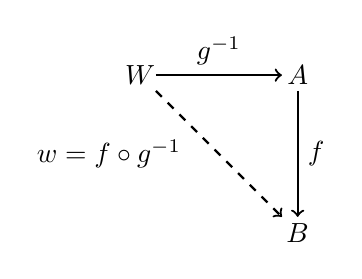
\begin{tikzpicture}
    \draw (0,0) node {$W$};
    \draw (2,0) node {$A$};
    \draw (2,-2) node {$B$};
    \draw[thick, ->] (0.2,0) -- (1.8,0) node[midway, above] {$g^{-1}$};
    \draw[thick, ->] (2,-0.2) -- (2,-1.8) node[midway, right] {$f$};
    \draw[thick, dashed, ->] (0.2,-0.2) -- (1.8,-1.8) node[midway, left=10pt] {$w = f \circ g^{-1}$};
  \end{tikzpicture}
\end{center}

This demonstrates that it is possible to write functions from finite sets to other finite sets, assuming that we can actually write functions like $f$ and $f^{-1}$ in lambda calculus. We begin with the function which takes a set $\{1,\ldots,n\}$ and map them to list of terms of the form $X_1\ldots X_n$.\\

It its simplest form, this function takes elements of the set $\{1,2\}$ and maps them into a list of length 2. We represent $1$ and $2$ with the terms:

\begin{eqnarray*}
  K_2^1 := \l x_1x_2.x_1\\
  K_2^2 := \l x_1x_2.x_2\\
\end{eqnarray*}

So our function consists of a list $\langle X_1,X_2 \rangle$, and takes either of the above functions. In general, we call terms like $\l x_1x_2.x_1$ $K_i^n$, where $n$ is the number of terms in the list, and $i$ is the index of the element we want from inside that list. We can generally define $K_n^i$ as the term\\
\begin{equation*}
  K_n^i := \l x_1\ldots x_n.x_i
\end{equation*}

So now let us say that we have a finite set $\{1,\ldots,n\}$, and we want to create the function $f:\{1,\ldots,n\} \rightarrow \{x_1,\ldots,x_n\}$. Hopefully, we can describe a term $T_f$ such that when we apply it to a term $K_i^n$, it is be beta equal to $K_{f(i)}^n$.
\begin{equation*}
  (T_fK_i^n) =_\beta K_{f(i)}^n
\end{equation*}

This now leaves us with the question of defining $T_f$. An easy way is to simply repeat our table lookup function scheme:
\begin{equation*}
  T_f := \l a.a(K_{f(1)}^nK_{f(2)}^n\ldots K_{f(n)}^n)
\end{equation*}

\examplebox{Example: Demonstration of $T_f$}{
\begin{equation*}
  T_fK_i^n \rightarrow_\beta K_i^n K_{f(1)}^n K_{f(2)}^n \ldots K_{f(n)}^n \twoheadrightarrow_\beta K_{f(i)}^n
\end{equation*}
}

Any function $f:\{1,\ldots,n\} \rightarrow \mathbb{S}$ can be created by this lookup table strategy. But what about functions of the form $f : \{1,\ldots,n\} \times \{1,\ldots,n\} \rightarrow \{1,\ldots,n\}$, or $f(i,j)$? To create functions of more than one variable, we can simply curry the inputs by definining $f_i(j) := f(i,j)$, and redefining $T_f := \l a.aT_{f_1}T_{f_2}\ldots T_{f_n}$.\\

We will defer discussion of the inverse functions until we have a chance to understand techniques for recusion and bounded search. For now, it is sufficient to say that they exist.
